\section{Stand der Technik}
\label{sec:Stand der Technik}

\subsection{Aktuelle Situation}
\label{sub:Aktuelle Situation}

In \ac{OSM} gibt es mehrere Arten, wie Mapper mit Flächen umgehen. So wirken einige Mapper dem Fussgängerrouting-Problem über Flächen mit zusätzlichen eingezeichneten Wegen entgegen, oder aber die Fläche ist ganz von Wegen befreit.

In Abbildung \ref{fig:helvetiaplatz_comparison} und Abbildung \ref{fig:sechselaeutenplatz_comparison} ist ein Vergleich gängiger Routing-Engines abgebildet, welche ein Fussgänger-Profil anbietet. In Abbildung \ref{fig:helvetiaplatz_comparison} sieht man schön, wie es bei \ac{OSM} möglich ist, dass die eingezeichneten Fusswege über den Platz genutzt werden. Diese Route entspricht offensichtlich nicht einem natürlichen Fussgänger-Verhalten, da normalerweise der direkte Weg über den Platz gewählt wird, sofern keine Hindernisse im Weg sind. An dieser Stelle scheitert Google Maps. Der Vergleich von Google Maps und \ac{OSM} hinkt hier natürlich, da nicht beide auf den genau gleichen Datenbestand zurückgreifen. Betrachtet man in Abbildung \ref{fig:sechselaeutenplatz_comparison} hingegen den Sechseläutenplatz, sieht man, dass ohne eingezeichnete Wege alle getesteten Anbieter um den Platz herum führen.

\begin{figure}[ht]
\centering
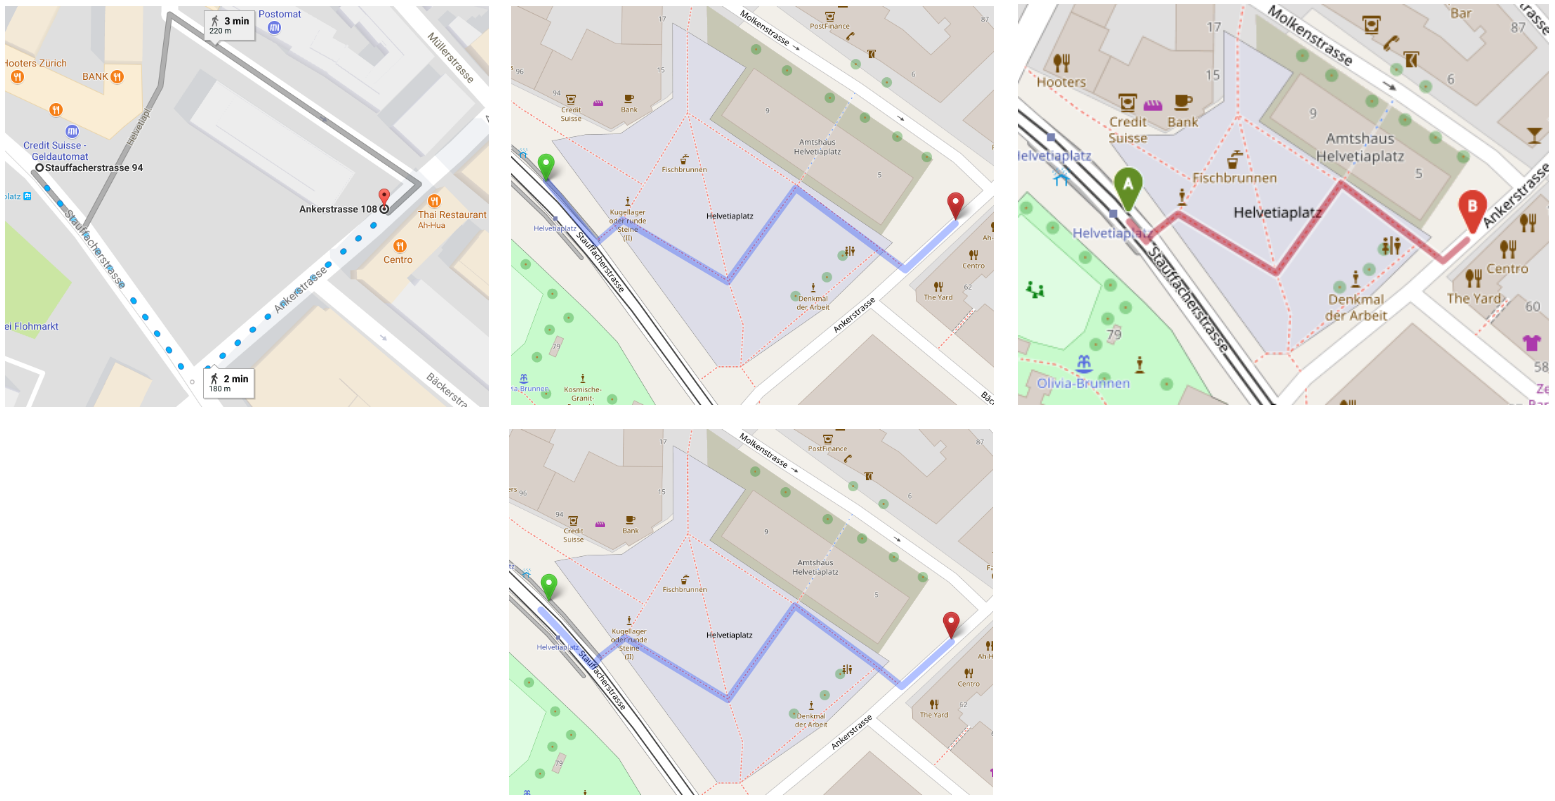
\includegraphics[width=1\linewidth]{technicalreport/img/helvetiaplatz_comparison}
\caption[Fussgänger-Routing Vergleich]{Routing-Vergleich von verschiedenen Anbietern mit Fussgänger-Profil über den Helvetiaplatz, Zürich, Schweiz; Links: Google Maps, Mitte-Oben: openstreetmap.org mit GraphHopper, Mitte-Unten: openstreetmap.org mit Mapzen, Rechts: openrouteservice.org; Screenshots aufgenommen am 13.10.2017}
\label{fig:helvetiaplatz_comparison}
\end{figure}

\begin{figure}[ht]
\centering
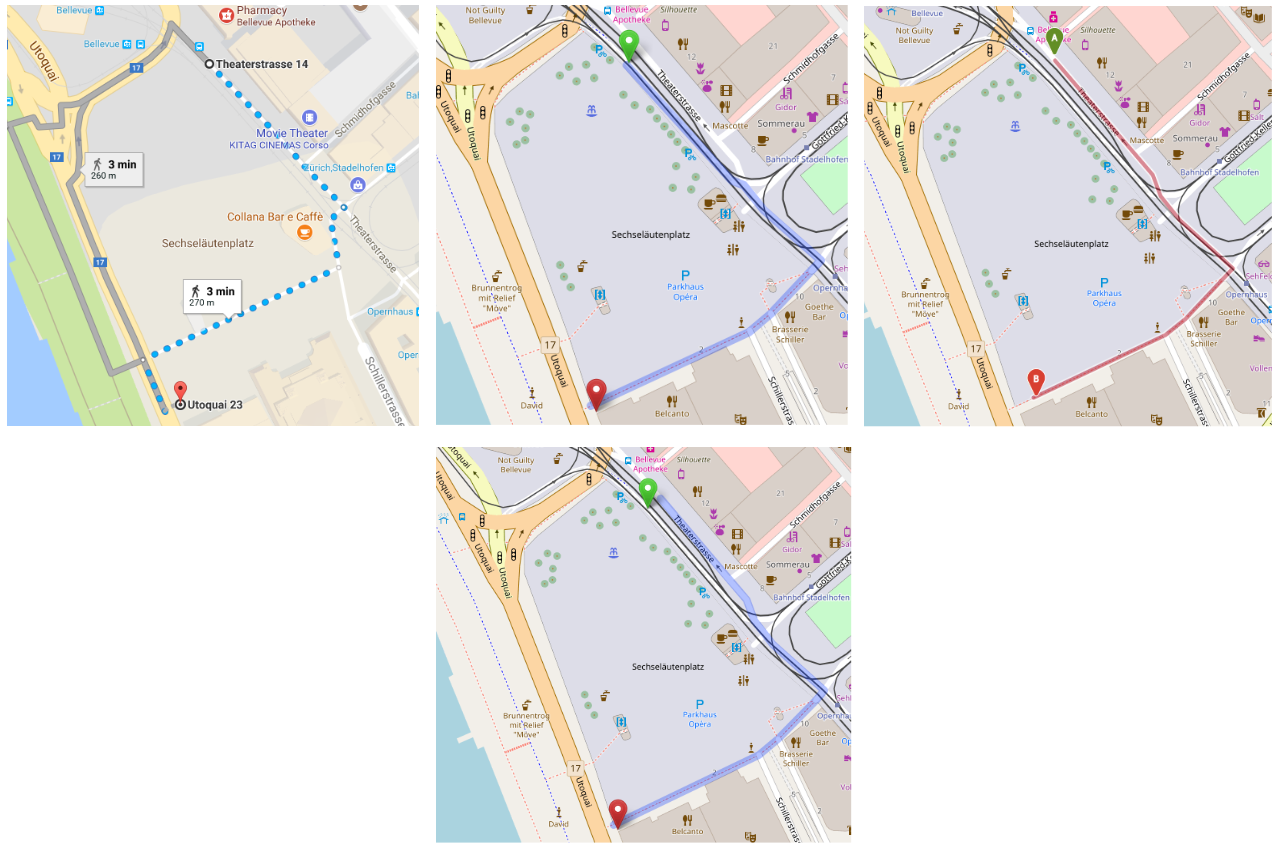
\includegraphics[width=1\linewidth]{technicalreport/img/sechselaeutenplatz_comparison}
\caption[Fussgänger-Routing Vergleich]{Routing-Vergleich von verschiedenen Anbietern mit Fussgänger-Profil über den Sechseläutenplatz, Zürich, Schweiz; Links: Google Maps, Mitte-Oben: openstreetmap.org mit GraphHopper, Mitte-Unten: openstreetmap.org mit Mapzen, Rechts: openrouteservice.org; Screenshots aufgenommen am 13.10.2017}
\label{fig:sechselaeutenplatz_comparison}
\end{figure}


Abschliessend kann man sagen, dass alle getesteten Routing-Engines mit den Fussgänger-Profilen mit Stand 13.10.2017 scheitern, wenn keine Wege über die Fläche eingezeichnet sind, und so die Dauer und Streckenlänge verfälscht wird.

\subsection{Lösungsansätze}
\label{sub:Lösungsansätze}


\subsubsection{Routing über offene Flächen}
\label{solution:Routing über offene Flächen}

In den folgenden Unterkapitel werden bestehende Lösungsansätze aus der Literatur diskutiert, die das Problem des Routings über offene Flächen, wie in Kapitel \ref{subsub:Routing bei zwei benachbarten Flächen} beschrieben, lösen sollen. Die beiden vielversprechendsten Ansätze Visibility-Graph und SpiderWeb-Graph werden in Kapitel \ref{sec:Bewertung Routing über offene Flächen} tiefergehend miteinander verglichen.

\paragraph{Visibility-Graph}\label{solution:Visibility-Graph}~\\
Ein Ansatz zur Verhinderung von Kollisionen auf Flächen wurde in \cite{lozano-perez_visibility_graph} als Visibility-Graph beschrieben. Dabei wird in einem ersten Schritt für jeden Knotenpunkt einer Fläche eine Verbindung zu jedem anderen Knotenpunkt gezeichnet. Für unsere Zwecke werden dabei alle Knotenpunkte eines Polygons, Hindernisse,  sowie Schnittpunkte mit Strassen und Wegen (\glspl{Einstiegspunkt}) beachtet.

In einem zweiten Schritt werden alle Verbindungen verworfen, die nicht komplett innerhalb der Fläche liegen oder mit einem Hindernis darauf kollidieren.

\begin{listing}[ht]
    \inputminted{python}{technicalreport/listing/visibility_graph_pseudocode.py}
    \caption{Konstruktion eines optimierten Visibility-Graphen}
    \label{visibility_graph_pseudocode}
\end{listing}

Für die Verwendung im Routing beschreibt \cite{graser_visibility_graph} einen Ansatz, um die Kanten des Visibility-Graphen zu reduzieren (siehe Listing \ref{visibility_graph_pseudocode}). Mit dem Visibility-Graphen allein gäbe es mit \(n\) Knotenpunkten bis zu \(n(n-1)/2\) Kanten. Für die Reduktion wird für jeden \gls{Einstiegspunkt} (wie aus Schritt 1 bekannt) jeweils der kürzeste Pfad auf dem Visibility-Graphen zu allen anderen Einstiegspunkten berechnet. Alle Kanten, die nicht zu einem kürzesten Pfad gehören, werden verworfen. Abbildung  \ref{fig:visibility_graph_comparison} zeigt einen Vergleich zwischen eines Visibility-Graphen vor und nach dem Reduktionsverfahren.

\begin{figure}
    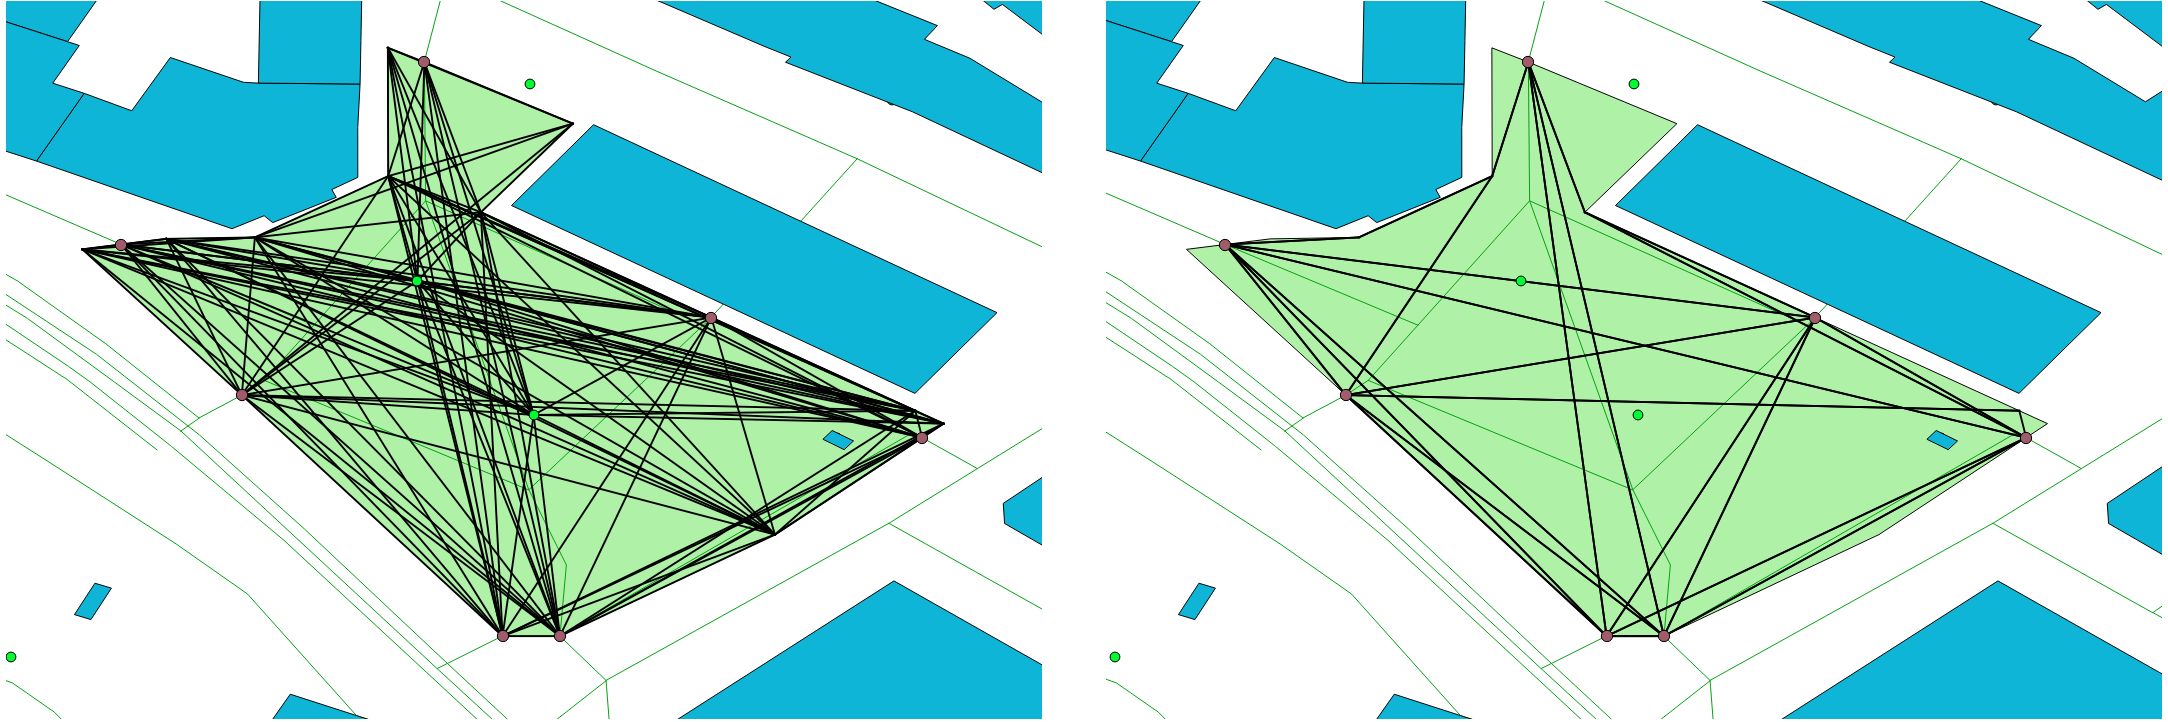
\includegraphics[width=\textwidth,keepaspectratio]{technicalreport/img/visibility_graph_comparison.png}
    \caption[Visibility-Graph über Helvetiaplatz]{Visibility-Graph über den Helvetiaplatz, Zürich, Schweiz; Links: Unveränderter Visibility-Graph; Rechts: Reduziert auf kürzeste Pfade}
    \label{fig:visibility_graph_comparison}
\end{figure}

\paragraph{SpiderWeb-Graph}\label{solution:SpiderWeb-Graph}~\\
Die Arbeit \cite{dzafic_spider_web_graph} befasst sich mit dem Flächenrouting für Nutzern von Elektrorollstühlen, indem ein Spinnennetz (siehe Abbildung \ref{fig:spiderweb}) über das Polygon gelegt wird. Dies hat den Vorteil, dass auf der Fläche zusätzliche Linien und Kanten vorhanden sind (wobei statische Hindernisse berücksichtigt werden), welche für das Routing verwendet werden können. Diese Idee und das Grundprinzip wurde im Folgenden übernommen.

\begin{figure}[ht]
\centering
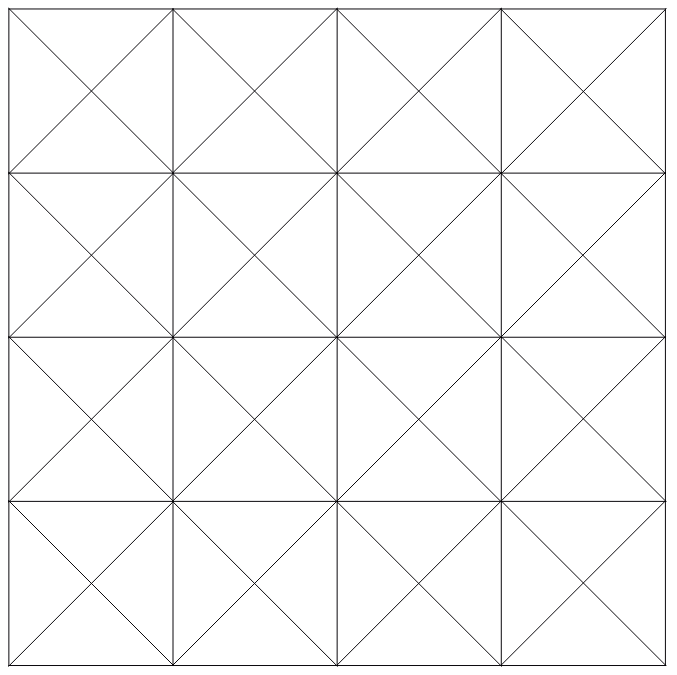
\includegraphics[width=0.5\linewidth]{technicalreport/img/spiderweb}
\caption[Spinnennetz]{Spinnennetz}
\label{fig:spiderweb}
\end{figure}

Auf dem Spinnennetz wird ähnlich wie beim \nameref{solution:Visibility-Graph} zwischen allen \glspl{Einstiegspunkt}n der Shortest-Path berechnet. Für die weitere Verarbeitung werden nur noch diese optimierten Pfade verwendet. Zur Verdeutlichung der Idee ist der Pseudocode in Listing \ref{SpiderWeb Pseudocode} zu betrachten.

\begin{listing}[ht]
    \inputminted{python}{technicalreport/listing/spiderweb_pseudocode.py}
    \caption{SpiderWeb Pseudocode}
    \label{SpiderWeb Pseudocode}
\end{listing}

Damit ein Spinnennetz über eine Fläche gezeichnet werden kann, muss eine Bounding-Box berechnet werden. Es handelt sich dabei um ein Rechteck, welches die ganze Fläche überdeckt. 

Vor dem Zeichnen des Spinnennetz ist es möglich, den Abstand zwischen Spalten und den Zeilen (Spacing) zu definieren. Dies hat hohe Auswirkung auf die Anzahl Zeilen und Spalten und somit auf die gezeichneten Pfade über die Fläche, da mit einem kleineren Spacing eine "Glättung" der Pfade möglich ist. Die gezeichneten Pfade widerspiegeln so eher das Verhalten eines Fussgängers. Ein Abstrich des kleiner Spacings ist sofort ersichtlich, wenn man das Spinnennetz in der Abbildung \ref{fig:spiderweb} betrachtet. Man kann annehmen, dass dieses Spinnennetz über eine Fläche von 4*4 cm mit einem Spacing von einem 1 cm gezeichnet wird. Verkleinert man nun das Spacing auf 0.5 cm, steigt die Anzahl der zu zeichnenden Linien von 72 auf 272. Halbiert man ein weiteres Mal, ist man bereits bei 1056 Linien. Damit ein Routing über das Spinnennetz und somit Abzweigungen möglich sind, kann nicht eine Line pro Zeile oder Spalte genutzt werden.

Das Zeichnen des Spinnennetzes hat eine Effizienz von \(O(N\times M)\), wobei N und M die Anzahl Spalten und Zeilen sind. Die Anzahl der Zeilen und Spalten erfahren beim Halbieren des Spacings jeweils ein quadratisches Wachstum. Durch ein kleineres Spacing steigen auch die Anzahl möglicher Pfade über die Fläche an, was Auswirkung auf die Dauer der Generierung des Shortest Paths hat. 

Betrachtet man das Resultat in Abbildung \ref{fig:spiderweb_result}, sieht man in Schwarz den generierten Shortest Path über die Fläche.

\begin{figure}[th]
\centering
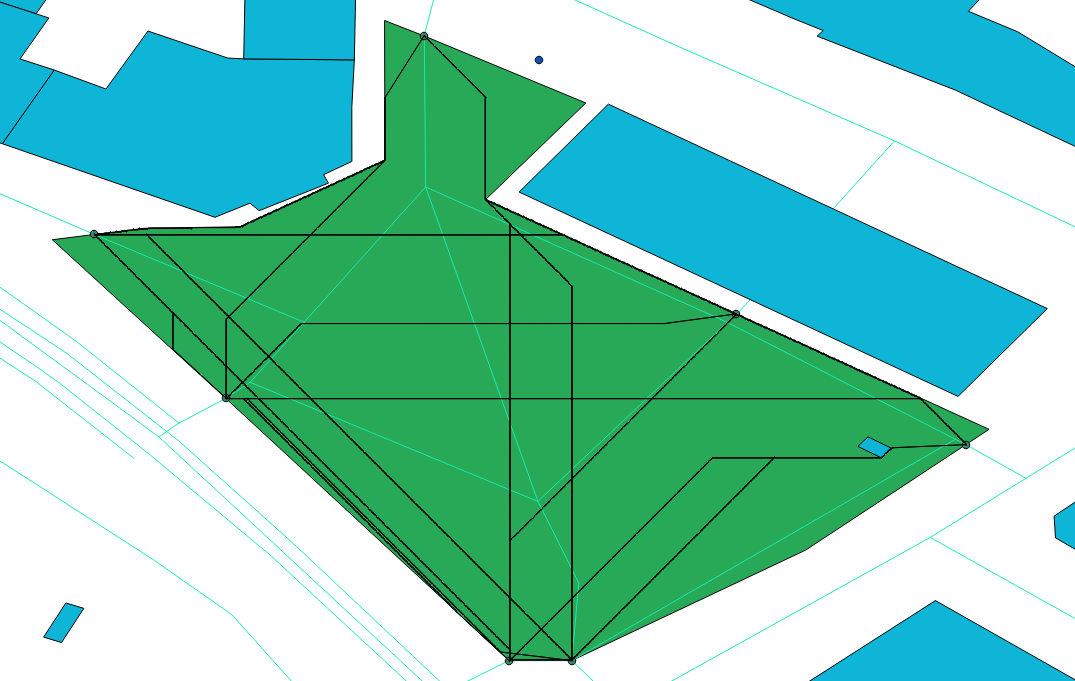
\includegraphics[width=0.7\linewidth]{technicalreport/img/spiderweb_result}
\caption[Resultat SpiderWeb-Graph]{Resultat SpiderWeb-Graph über Helveltiaplatz, Zürich, Schweiz}
\label{fig:spiderweb_result}
\end{figure}


Es wurde ebenfalls geprüft, ob die Rotation des Spinnennetz auf die Gegebenheit der Fläche eine Auswirkung auf die Shortest Path-Generierung hat. Bei einem Test, welcher in Abbildung \ref{fig:rotation_comparison} ersichtlich ist, wurden keine entscheidenden Vorteile gefunden, warum sich der zusätzliche Aufwand rechtfertigen würde. Das Spinnennetz wurde um 45 und um 90 Grad gedreht. Die berechneten kürzesten Pfade sind fast identisch.

\begin{figure}[th]
\centering
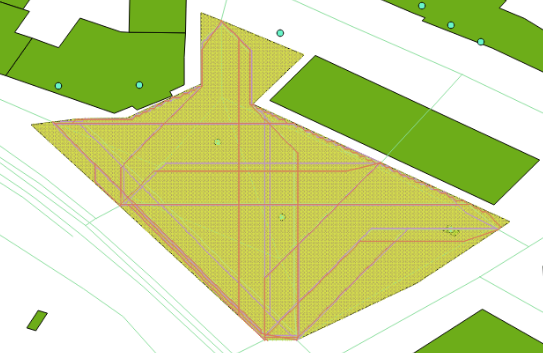
\includegraphics[width=0.7\linewidth]{technicalreport/img/rotation_comparison}
\caption[SpiderWeb-Graph Vergleich mit Rotation]{Rotation des SpiderWebs um 45 und 90 Grad im Vergleich mit keiner Rotation}
\label{fig:rotation_comparison}
\end{figure}

\paragraph{Straight Skeleton}~\\
Die Methode vom \emph{Straight Skeleton} wurde erstmals in \cite{aichholzer_skeleton} eingeführt. Dabei werden Schritt für Schritt die Kanten des Polygons zur Mitte zusammen geführt, es entstehen Verbindungen mit scharfen Ecken zu den Eckpunkten des Polygons. In Abbildung \ref{fig:skeleton_example} ist beispielhaft ein Graph aufgezeichnet.

Die Andwendung dieser Methode für Flächenrouting wurde bereits in \cite{graser_visibility_graph} diskutiert. Es stellt sich heraus, dass die \emph{Straight Skeleton} Methode keine natürlichen Routen für Fussgänger ergibt, da sie tendenziell zur Mitte der Fläche gehen und sich dabei scharfe Kurven ergeben. Aus diesen Gründen wird dieser Ansatz nicht weiter behandelt.

\begin{figure}[th]
\centering
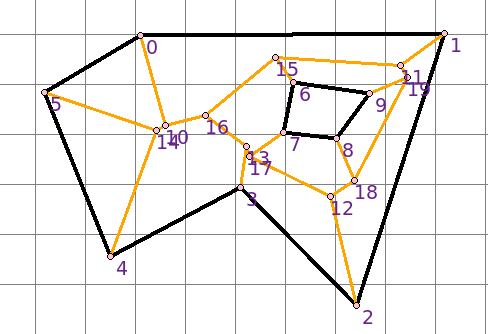
\includegraphics[width=0.7\linewidth]{technicalreport/img/skeleton_example.png}
\caption[Straight Skeleton Beispiel]{Straight Skeleton eines Multipolygons; Erstellt mit der Software pySkeleton von Ecole Centrale Paris}
\label{fig:skeleton_example}
\end{figure}


\subsubsection{Routing über über weitere Arten von offenen Flächen (Berge, Strände)}
\label{subsub:Routing über über weitere Arten von offenen Flächen (Berge, Strände)}

Wie in \ref{problem:Routing über über weitere Arten von offenen Flächen (Berge, Strände)} beschrieben, ergeben sich beim Überqueren von offenen Landflächen wie Berge oder Strände andere Fragestellungen. Hier spielt die Unterlage eine grössere Rolle, Faktoren wie Höhe oder Beschaffenheit des Untergrunds sind nun relevant. Für diese Problematik wird ein technischer Lösungsansatz vorgestellt und bewertet.

\paragraph{Technischer Ansatz mit Cost Path Analyse}~\\
Ein Ansatz für die Berechnung von Routen über offene Flächen ist die Cost Path Analyse \cite{cost_path_analysis}. Dieses Verfahren wird oft angewendet, um in einer Fläche Korridore zu finden, um darin beispielsweise neue Strassen zu erschliessen \cite{gis-wiki:cost-path-analysis}.

In einem ersten Schritt wird ein Raster über die Fläche gelegt. Jeder Kachel wird ein Wert zugewiesen, der den Kosten entspricht, um diese Fläche zu traversieren. Die Kosten können zusammen gesetzt sein aus mehreren Faktoren wie die Steigung oder Beschaffenheit des Untergrunds. So bekäme etwa ein Sandstrand höhere Kosten als eine Asphalt-Fläche. Dieses Raster wird auch Cost Surface genannt. \cite{gid_fundamentals}

Sobald ein Startpunkt der Route bekannt ist, kann als nächstes ein Cost Distance Raster erstellt werden. Mit Hilfe der Cost Surface wird im Raster vom Startpunkt aus zu jedem erreichbaren Punkt die minimalen Kosten akkumuliert \cite{geospatial_analysis}. Ist nun der Zielpunkt der Route ebenfalls bekannt, kann von diesem Zielpunkt aus jeweils zur Nachbar-Kachel mit den geringsten Kosten navigiert werden, bis der Startpunkt erreicht wurde \cite{cost_path_analysis}. In Abbildung \ref{fig:cost_path_analysis} ist eine Cost Path Analyse beispielhaft dargestellt.


\begin{figure}[ht]
    \centering
    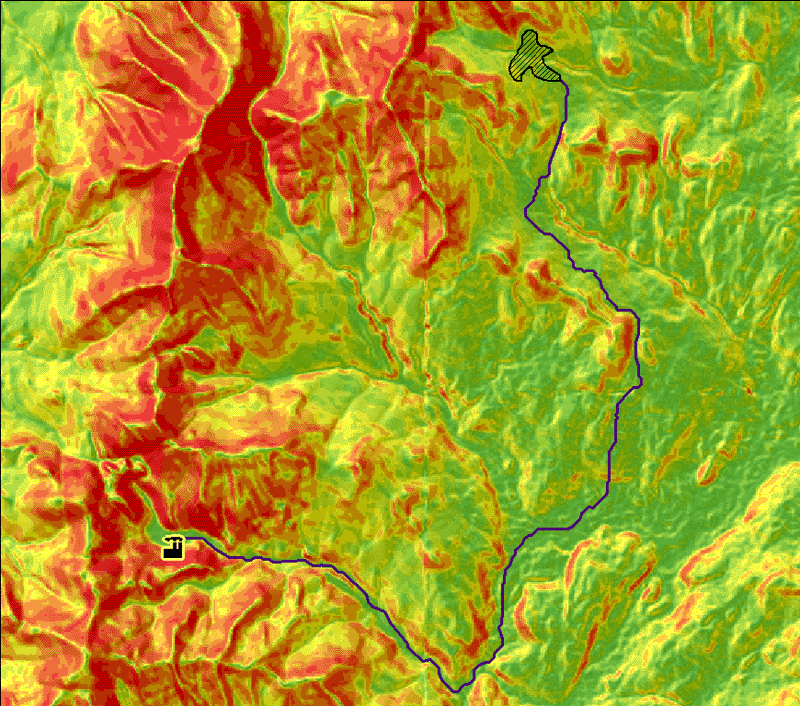
\includegraphics[width=0.6\linewidth]{technicalreport/img/cost_path_analysis}
    \caption[Cost Path Analyse]{Resultat einer Cost Path Analyse; Grafik von \cite{geospatial_analysis}}
    \label{fig:cost_path_analysis}
\end{figure}

\paragraph{Bewertung}~\\
Im Kontext des Fussgänger-Routings gibt es mit dem Ansatz der Cost Path Analyse einige weitere Fragestellungen. Für jede Fläche müsste zuerst eine Cost Surface erstellt werden. Das Cost Distance Raster kann dann erst zur Laufzeit berechnet werden, da Start- und Zielpunkt vorher nicht bekannt sind.

Bei offenen Landflächen in Bergen ist es ausserdem schwierig zu entscheiden, ob ein Fussgänger eine Fläche passieren kann. Solche Flächen sind in \ac{OSM} oft nicht gemappt und es besteht keine Information über den Untergrund. Es kommen auch andere Faktoren wie z.B. die Jahreszeit hinzu. So könnte das Begehen einer Wiese im Sommer problemlos, im Winter aber durch eine Schneedecke zeitweise unmöglich sein. Bei Stränden sieht es wiederum anders aus, diese sind in \ac{OSM} meist als Flächen gemappt. Dort spielt aber auch das Höhenprofil normalerweise keine Rolle, womit ein Ansatz wie unter \ref{solution:Routing über offene Flächen} wieder effizienter sein könnte.


\subsubsection{Datenaufbereitung für das Fussgänger-Routing über Strassen}
\label{subsub:Datenaufbereitung für das Fussgänger-Routing über Strassen}

Damit eine Routing-Engine die Kartendaten für das Routing nutzen kann, müssen diese zuerst zu einem Graphen aufbereitet werden. Für das Fussgänger-Routing ergeben sich dabei andere Herausforderungen als beispielsweise bei motorisiertem Individualverkehr. So muss etwa beim Fussgänger-Routing beachtet werden, wann ein Fussgänger die Strasse überqueren kann. Dafür müssen gewisse Annahmen getroffen werden. Eine kaum befahrene Strasse in einem ländlichen Gebiet kann höchstwahrscheinlich jederzeit überquert werden, während in einem städtischen Gebiet eher Fussgängerstreifen verwendet werden.

Ein wichtiger Bestandteil der Datenaufbereitung ist der Einbezug von Bürgersteige. Diese werde in OpenStreetMap auf unterschiedliche Weise gemappt \cite{osm_wiki_sidewalks}. Sie können als eigene Wege oder als Eigenschaft der Strasse definiert werden. In \cite{pedestrian_navigation_lang} wurde ein Datenmodell für Fussgänger-Routing entwickelt. Dabei ist die Datenqualität der \ac{OSM}-Daten bei Bürgersteigen weiterhin ein Problem. In den letzten Jahren gab es Bemühungen, die Datenqualität von Bürgersteige \cite{mapbox_sidewalk_improving} und Fussgängerstreifen \cite{crosswalks_aerial_extraction} durch die Analyse von Sattelitenbilder zu verbessern.

Abschliessend kann man sagen, dass die Datenaufbereitung für Fussgänger-Routing weiterhin eine Herausforderung ist. Auch wenn diese für die Hauptproblemstellung von Routing über offene Flächen nicht direkt relevant sind, ist dies ein wichtiger Bestandteil für das Fussgänger-Routing als Ganzes.


\subsubsection{Start-/Endpunkt auf der Fläche}
\label{subsub:Start-/Endpunkt auf der Fläche}
Ein Spezialfall des Fussgänger-Routings entsteht, wenn der Start- oder Endpunkt auf einer Fussgänger-Fläche liegt. Wie in \ref{problem:Start-/Endpunkt auf der Fläche} beschrieben ist es üblich, dass Routing-Engines eine Mittelsenkrechte zum nächten Punkt auf dem Strassennetz ziehen.

In unserem Prototyp erfolgt die komplette Berechnung der kürzesten Wege durch Fussgänger-Flächen im Voraus, zur Laufzeit (bei einer Anfrage des Benutzers) werden die neu berechneten Fusswege lediglich von der Routing-Engine verwendet. Für unsere Zwecke ergeben sich so zwei mögliche Ansätze:

\begin{enumerate}
    \item Zur Laufzeit wird vom Start-, bzw. Endpunkt auf der Fläche der kürzeste Weg zum Strassennetz in Richtung der Route berechnet, dabei werden Hindernisse umgangen.
    \item Die von uns berechneten Wege über Flächen reichen aus, die Routing-Engine zieht eine Mittelsenkrechte auf den nächstgelegenen Fussweg auf der Fläche. Zur Laufzeit müssen keine zusätzlichen Berechnungen durchgeführt werden.
\end{enumerate}

\begin{figure}[ht]
    \centering
    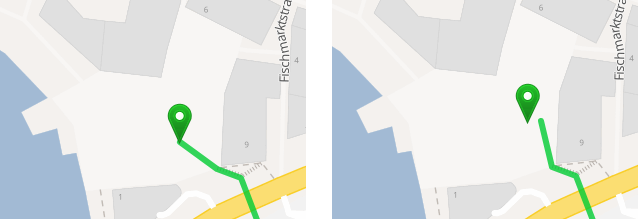
\includegraphics[width=1\linewidth]{technicalreport/img/vergleich_start-punkt-auf-flaeche}
    \caption[Vergleich der Ansätze wenn Startpunkt auf Fläche]{Vergleich einer beispielhaften Route mit dem Ansatz 1 (links) und Ansatz 2 (rechts); Gezeigt auf dem Fischmarktplatz, St. Gallen, Rapperswil; Screenshot von Graphhopper \cite{graphhopper}}
    \label{fig:vergleich_start-punkt_auf_fläche}
\end{figure}


Wie in Abbildung \ref{fig:vergleich_start-punkt_auf_fläche} zu sehen, ergibt der zweite Ansatz ohne zusätzlichen Berechnungen genügend gute Resultate, da es zwischen jedem Ein- und Ausgangspunkt ein Fussweg hat, der bereits den kürzesten Weg beschreibt. Eine zusätzliche Berechnung des kürzesten Pfades wie im ersten Ansatz ergibt keine signifikante Verbesserung der Route.

\subsubsection{Routing bei zwei benachbarten Flächen}
\label{subsub:Routing bei zwei benachbarten Flächen}

Wie in \ref{target:Routing bei zwei benachbarten Flächen} beschrieben, gibt es bei zwei benachbarten Flächen einen Spezialfall für das Routing. Bei unserer Implementation wissen die beiden Flächen nichts voneinander und es werden keine \glspl{Einstiegspunkt} erkannt, wo der Fussgänger die Abgrenzung der beiden Flächen überqueren könnte.

Im Rahmen unserer Arbeit haben wir in der Literatur keine entsprechende Diskussion dazu gefunden. Wir haben für die Lösung des Problems zwei Ansätze überlegt:

\begin{enumerate}
    \item Die beiden Flächen miteinander kombinieren: Wenn sich zwei Fussgänger-Flächen berühren, können sie geometrisch vereint und als eine einzige Fläche angesehen werden.
    \item Gemeinsame \glspl{Einstiegspunkt} zwischen den Flächen definieren: An der Kante, wo sich zwei Flächen berühren, werden künstlich in einem regelmässigen Abstand Einstiegspunkte eingefügt, wo für das Routing der Fussgänger die Kante überqueren kann.
\end{enumerate}

\subsection{Verbesserungsmöglichkeiten}
\label{sub:Verbesserungsmöglichkeiten}
% Hinweise auf Weiterentwicklungs-, bzw. Verbesserungspotential
Für die in Kapitel \ref{sub:Lösungsansätze} diskutierten Ansätze für Routing über offene Flächen werden Defizite und mögliche Verbesserungsmöglichkeiten aufgezeigt.

\subsubsection{Einstiegspunkte}
\label{subsub:Verbesserung_Einstiegspunkte}

Sowohl der \nameref{solution:SpiderWeb-Graph} wie auch der \nameref{solution:Visibility-Graph} benutzen \glspl{Einstiegspunkt}, um die kürztesten Pfade zu finden und den Graphen mit dem bestehenden Strassennetz zu verbinden. Es kommt allerdings oft vor, dass es auf einer Fussgängerfläche keinen oder nur einen einzigen Einstiegspunkt gibt, wodurch auch kein Graph berechnet werden kann. In der Realität könnte es aber trotzdem möglich sein, eine solche Fläche zu Fuss zu überqueren, auch wenn keine Strasse daran angrenzt.

Eine mögliche Lösung dieses Problems könnte sein, die Umgebung der Fussgänger-Fläche zu analysieren und künstliche \glspl{Einstiegspunkt} dort einzufügen, wo ein Fussgänger die Fläche betreten kann. Dies könnte von einer angrenzenden Fussgänger-Fläche aus sein (siehe Kap. \ref{subsub:Routing bei zwei benachbarten Flächen}) oder von einer anderen Fläche, wobei der Zutritt zur Fussgänger-Fläche nicht durch ein Hinderniss verunmöglicht werden soll.

\subsubsection{SpiderWeb-Graph}
\label{subsub:Verbesserung_SpiderWeb}

Ein Problem des SpiderWeb-Graphen ist die Auflösung des Gitters (SpiderWebs), die gewählt werden muss, um optimale Routen zu erhalten. Bei einer zu kleinen Auflösung macht die Route viele Kurven, da sie ständig dem Gitter entlang fahren muss. Eine sehr grosse Auflösung des SpiderWebs ist aber für die Praxis sehr rechenaufwändig, da die benötigte Rechenzeit quadratisch mit einer höheren Auflösung steigt.

Eine mögliche Verbesserung für dieses Problem ist die Anwendung einer Glättung auf die erzeugte Route. Damit wird die Anzahl der Kurven verringert und so einen natürlicheren Pfad erzeugt. Ein Ansatz dafür bietet der Douglas-Peucker Algorithmus \cite{douglas-peucker_algorithm}, der eine Linien-Geometrie vereinfachen kann. Dabei muss allerdings sichergestellt werden, dass die Glättung der Route nicht mit einem Hinderniss kollidiert oder ausserhalb der Fläche fällt. Mit Hilfe der Glättung kann so eine kleinere Auflösung für das SpiderWeb gewählt werden, was zusätzlich Rechenzeit spart.